% =============================================================================
% paper.tex — "A Priority That Does Not Bind"
% Journal of Population Economics submission draft.
% Compile with pdfLaTeX + BibTeX (paper -> bibtex paper -> paper -> paper).
% =============================================================================
\documentclass[12pt]{article}

\usepackage[utf8]{inputenc}
\usepackage[T1]{fontenc}
\usepackage{times}
\usepackage[margin=1in]{geometry}
\usepackage{setspace}
\usepackage{booktabs}
\usepackage{graphicx}
\usepackage{amsmath}
\usepackage{amssymb}
\usepackage{caption}
\usepackage{float}
\usepackage{xcolor}
\definecolor{citegreen}{RGB}{0,120,60}
\usepackage[colorlinks=true,citecolor=citegreen,urlcolor=citegreen,linkcolor=citegreen]{hyperref}
\usepackage[round]{natbib}
\bibliographystyle{plainnat}

\graphicspath{{../analysis/output/graphs/}{../analysis/output/maps/}}
\captionsetup{font=small,labelfont=bf}
\onehalfspacing

\title{\textbf{A Priority That Does Not Bind:\\ Telework Mandates and Mothers of Young Children in Brazil}}
\author{Fredie Didier\thanks{Instituto Brasileiro de Ensino, Desenvolvimento e Pesquisa (IDP), Bras\'ilia, Brazil. E-mail: fdidier@terra.com.br.}}
\date{\today}

\begin{document}
\maketitle

\begin{abstract}
\noindent In 2022, Brazil enacted a law requiring employers to give employees with children under 4 years old \emph{priority} in the allocation of positions eligible for telework. Because the law grants a priority rather than an enforceable right, it need not translate into more telework in practice. Using quarterly rotating panel data from the Continuous National Household Sample Survey (PNAD Cont\'inua) for 2018--2026, and a difference-in-differences design that compares mothers of children under 4 to mothers of children aged 5--7, I find no effect on the share of women working from home. The null holds across specifications, subgroups, and robustness checks, and there is no sign that eligible mothers moved into telework-friendly occupations. The evidence indicates that a discretionary, unenforceable priority did not change the outcome it targeted.

\vspace{0.5em}
\noindent\textbf{Keywords:} telework; work from home; gender; family policy; child penalty; Brazil

\vspace{0.3em}
\noindent\textbf{JEL codes:} J13; J16; J22; J18; K31
\end{abstract}

\clearpage

% =============================================================================
\section{Introduction}
% =============================================================================

The arrival and persistence of a young child remains one of the sharpest turning points in a woman's working life. Across high- and middle-income countries, mothers' earnings and employment fall abruptly at the birth of a first child and recover slowly, if at all, while fathers' trajectories are largely undisturbed \citep{kleven2019denmark,kleven2019countries}. In Brazil the tension between paid work and young children is severe: women's labor-force participation stands roughly 20 percentage points below men's, women perform close to twice as many weekly hours of unpaid domestic work and caregiving, and the employment rate of mothers with a child under 3 is well below that of women without young children \citep{ibge_gender}. At the same time, the pandemic made working from home a mainstream possibility for a meaningful minority of jobs and put workplace flexibility at the center of the policy debate on gender gaps \citep{barrero2023,dingelneiman2020}. Whether flexibility can be legislated into the hands of the workers who need it most is, therefore, a first-order question for population and family economics.

Economic theory offers a clear reason to expect flexibility to matter and an equally clear reason to doubt that a soft legal instrument can deliver it. On the demand side, \citet{goldin2014} argues that a large part of the remaining gender gap reflects the disproportionate reward that firms attach to long, inflexible hours, so that arrangements which relax the time constraint, telework prominent among them, are precisely what could narrow it. Workers, in turn, value such arrangements: \citet{maspallais2017} show that the average worker is willing to give up a non-trivial fraction of wages to avoid rigid schedules, and \citet{bloom2015} document that home work can raise, rather than lower, productivity. Yet the instrument at issue here is not a subsidy or an entitlement but a mandated \emph{priority}, and the economics of mandated benefits warns that such mandates bind only weakly when compliance is costly and hard to verify \citep{summers1989,gruber1994}. When the law merely instructs employers to ``prioritize'' a group for a benefit that many jobs cannot supply, and provides no enforcement, standard incidence logic predicts little movement in equilibrium allocations.

This paper provides the first evidence on whether Brazil's telework-priority mandate changed the labor-market outcomes of the women it was meant to protect. In March 2022, through Provisional Measure 1108 and later Law 14.442, Brazil amended the Consolidation of Labor Laws (Article 75-F) to require employers to give priority in the allocation of telework-eligible positions to employees with children or legal dependents up to 4 years of age.\footnote{Provisional Measures have the force of law on publication; Provisional Measure 1108 took effect on 28 March 2022 and was converted, without change to Article 75-F, into Law 14.442 on 2 September 2022. The reform has therefore been in force since the end of the first quarter of 2022, which motivates treating the second quarter of 2022 as the first post-reform period. See \href{https://www.planalto.gov.br/ccivil_03/_ato2019-2022/2022/mpv/mpv1108.htm}{Provisional Measure 1108/2022} and \href{https://www.planalto.gov.br/ccivil_03/_ato2019-2022/2022/lei/l14442.htm}{Law 14.442/2022}.} I evaluate the reform using the rotating panel of the Continuous National Household Sample Survey (PNAD Cont\'inua), which follows individuals for up to 5 consecutive quarters and, since 2018, records whether each worker performs her main job at home.

The design compares women whose youngest child is under 4, who are eligible for the priority, with women whose youngest child is aged 5--7, who are similar in their selection into motherhood but just above the statutory threshold, in a difference-in-differences framework around the reform, with individual fixed effects that absorb time-invariant selection into motherhood. The main outcome is whether a woman works from home. This is the compliance proxy, or first stage: it measures how much the mandate actually moved telework take-up among eligible women, and so bounds any downstream effect on earnings, hours, or fertility. The estimate is an intent-to-treat effect, since I observe legal eligibility rather than whether any employer granted telework; it therefore recovers the effect of being entitled to priority, the policy-relevant parameter.

I find no effect. The share of eligible women working from home did not rise relative to the comparison group after the reform: the difference-in-differences estimate is $-0.1$ percentage points on a pre-reform base of about 5\%, and at the 95\% level I can rule out increases larger than about 0.5 percentage points. An event study shows flat pre-reform trends, including through the 2020--2021 pandemic, and, at most, a small effect emerging only two to three years later. A placebo supports the design: mothers whose youngest child is 5--7, whom the law does not cover, show no change relative to women with no young children at all, so it is the age-4 threshold, and not a broader difference between mothers and other women, that identifies the effect.

Additional results show that the null does not mask offsetting responses. The effect on home office remains zero even among women who were already in telework-eligible occupations at baseline, the only women for whom a priority over telework positions could bind, and treated mothers did not move into telework-eligible occupations after the reform, so there is no ``priority-seeking'' occupational sorting. The effect is likewise indistinguishable from zero across subgroups: for formal and informal workers, for registered private-sector employees (the group the statute binds) and public employees, and across education and age. The null survives alternative treatment and control definitions, dropping the pandemic years, state-by-quarter fixed effects, and alternative clustering. It is also robust to a triple-differences design that adds men with young children as a third comparison group: because the statute is gender-neutral, these men are themselves eligible, so comparing women's response to theirs nets out any generic shock to parents of young children after 2022 and isolates the woman-specific response. The absence of an effect is not gendered.

The pattern points to an institutional explanation. A priority is not a right: it is only as valuable as the stock of teleworkable positions an employer has to allocate, and for most eligible women, who work informally, in the public sector, or in jobs that cannot be done from home, that stock is close to empty. Section~\ref{sec:discussion} develops this reading and weighs it against alternatives.

The paper speaks to three literatures. The first is the economics of gender and workplace flexibility. \citet{goldin2014} argues that a large part of the remaining gender gap reflects the premium that firms place on long, inflexible hours, so that arrangements which relax the time constraint, telework foremost among them, are natural candidates to narrow it. Workers value such flexibility \citep{maspallais2017}, home-based work need not lower productivity \citep{bloom2015}, and the pandemic durably raised its prevalence \citep{barrero2023,dingelneiman2020}. Against this backdrop, a recurring hope is that widening access to flexible arrangements can compress gender gaps \citep{bertrand2011,blaukahn2017}; the present evidence shows that access cannot be legislated into existence when the underlying jobs are not teleworkable and compliance is voluntary.

Second, the paper contributes to the literature on the effectiveness of family policy and its relation to the child penalty \citep{kleven2019denmark,kleven2019countries,addadustmann2017,olivettipetrongolo2017}. This work has largely evaluated leave, cash transfers, and childcare. Telework priority is a newer and far cheaper instrument that governments increasingly reach for, and evidence on whether it works is scarce; documenting that a well-identified version of it moved neither telework take-up nor labor-market outcomes is directly useful for the design of family and flexible-work policy.

Third, the paper adds to the economics of group-specific mandated benefits and their enforcement \citep{summers1989,gruber1994}. This literature has shown that a mandate targeted at an identifiable group can shift that group's wages or employment. The present case sits at the opposite pole: a benefit so weakly binding, and so poorly matched to the jobs the target group actually holds, that it moves nothing. It does so in a middle-income labor market with a large informal sector and limited enforcement \citep{ulyssea2018,gerardgonzaga2021}, precisely the setting where soft mandates are most likely to fall flat.

The remainder of the paper is organized as follows. Section~\ref{sec:background} describes the reform and the institutional setting, Section~\ref{sec:data} the data and sample, and Section~\ref{sec:strategy} the empirical strategy. Section~\ref{sec:results} presents the results: the first stage, the reduced-form outcomes, the mechanisms, the heterogeneity analysis, and the robustness checks and triple difference. Section~\ref{sec:discussion} discusses the findings and Section~\ref{sec:conclusion} concludes.

% =============================================================================
\section{Institutional background}\label{sec:background}
% =============================================================================

Telework had no dedicated place in Brazilian labor law until 2017, when a broad labor reform introduced a chapter regulating remote work in the Consolidation of Labor Laws (CLT). The arrangement remained marginal until the pandemic forced a temporary and massive shift to home-based work in 2020--2021. As that shock receded, the federal government issued Provisional Measure 1108 on 25 March 2022 (published 28 March 2022), which modernized the telework chapter and, in its Article 75-F, created the provision studied here. The Provisional Measure was converted, with the same article, into Law 14.442 on 2 September 2022.

Article 75-F instructs employers to give \emph{priority} to employees with disabilities and to employees with children or legal dependents up to four years of age in the allocation of positions for activities that can be performed through telework or remote work. Three features of the provision shape the analysis. First, it is a priority in allocation, not a right to telework: the employer must place eligible employees ahead of others when distributing positions that are already teleworkable, but is not obliged to create such positions or to grant remote work to any particular employee. Second, it carries no dedicated enforcement mechanism or penalty and does not depend on employee request or certification. Third, it applies to employees under the CLT---formal, registered, private-sector and comparable workers---and not to the self-employed, employers, or the large set of workers without a registered contract. These features make the provision a near-textbook example of a soft mandate, and they motivate both the intent-to-treat interpretation and the placebo splits by contract type reported below.

% =============================================================================
\section{Data}\label{sec:data}
% =============================================================================

The analysis uses the Continuous National Household Sample Survey (PNADC), the rotating quarterly household survey conducted by the Brazilian Institute of Geography and Statistics (IBGE). PNADC interviews each selected household in up to 5 consecutive quarters, which yields a short panel at the individual level. I use all quarters from the first quarter of 2018---the first period in which the survey records the location where each worker performs her main job---through the first quarter of 2026. Individuals are linked across quarters using the survey's household and person identifiers together with an advanced matching procedure that reconstructs the panel even when interviews are incomplete; Appendix~\ref{app:pnadc} describes the survey and the panel construction in detail, and Appendix Table~\ref{tab:panel_retention} documents that the resulting panel captures genuine repeated observations of the same individuals and households.

The estimation sample consists of women aged 18--49 who are the head of the household or the head's spouse or partner---the group for whom the presence of a young child in the household is informative about their own children---and whom the panel algorithm links across quarters. The roughly 3.7\% of women who cannot be linked receive a singleton identifier and so contribute nothing under individual fixed effects; they are excluded, leaving the linked panel as the estimation sample. The key outcome is an indicator for working from home, defined as performing the main job at the worker's own residence. Additional outcomes are real monthly labor earnings, usual weekly hours, indicators for employment and labor-force participation defined over the full sample, and an indicator for being on maternity leave, a proxy for a recent birth. All statistics use the survey sampling weights.

Treatment is defined by the presence of a child aged 4 or younger in the household of a woman who is head or spouse. The primary comparison group consists of women with no child under 4 but with a youngest child aged 5--7: mothers who are similar on the margins that select women into motherhood but whose youngest child has just crossed the statutory age cutoff. A broader comparison group---women with no child aged 0--7---is used to gauge power and to construct a placebo. An occupation is classified as telework-eligible following the adaptation of \citet{dingelneiman2020} to Brazilian occupation codes in \citet{goes2020} and \citet{costa2024}; this classification is used as a moderator and as an outcome in the mechanism analysis, never as a sample restriction, because occupation may itself respond to the policy.

Table~\ref{tab:descriptives} reports summary statistics by group and period. Two patterns stand out. Working from home is uncommon in all groups---about five percent before the reform---and rises only modestly afterward, in parallel across groups. Treated women are younger, participate less in the labor market, and are less likely to hold a formal job than the comparison groups, exactly the selection that the individual fixed effects are meant to absorb.

\begin{table}[htbp]
\centering
\caption{Summary Statistics by Treatment Group}
\label{tab:descriptives}
\small
\begin{tabular}{lcccccc}
\toprule
 & \multicolumn{2}{c}{Treated (child $\leq$ 4 years)} & \multicolumn{2}{c}{Control A (child 5--7 years)} & \multicolumn{2}{c}{Control B (no child 0--7 years)} \\
\cmidrule(lr){2-3} \cmidrule(lr){4-5} \cmidrule(lr){6-7}
 & Pre-MP & Post-MP & Pre-MP & Post-MP & Pre-MP & Post-MP \\
\midrule
Home office (%) & 4.6 & 5.9 & 5.3 & 6.1 & 4.9 & 6.0 \\
In labor force (%) & 59.7 & 58.5 & 68.8 & 68.7 & 73.9 & 76.0 \\
Employed (%) & 84.8 & 90.9 & 86.7 & 92.0 & 88.5 & 93.0 \\
Habitual income (R$, real) & 2979 & 3099 & 2839 & 3133 & 3020 & 3204 \\
Usual weekly hours & 36.7 & 37.1 & 37.1 & 37.4 & 38.4 & 38.9 \\
Effective weekly hours & 33.0 & 34.4 & 34.7 & 36.0 & 35.9 & 37.5 \\
On maternity leave (%) & 1.8 & 1.7 & 0.1 & 0.1 & 0.1 & 0.1 \\
Formal employment (%) & 29.0 & 30.0 & 33.3 & 36.0 & 39.6 & 43.2 \\
Potential telework occupation (%) & 15.7 & 17.3 & 17.9 & 20.3 & 21.0 & 23.9 \\
Age (years) & 31.9 & 32.2 & 35.1 & 35.5 & 38.1 & 37.8 \\
\midrule
Observations & 357,588 & 338,856 & 168,866 & 171,644 & 779,904 & 773,094 \\
\bottomrule
\end{tabular}
\begin{tablenotes}
\small
\item \textit{Notes:} Sample restricted to women aged 18--49 who are household head or spouse, with at least one interview from 2018 onwards. Means are weighted using survey sampling weights. Post-MP refers to the second quarter of 2022 onwards. Treated women have a youngest child aged 0--4 in the household; Control A women have a youngest child aged 5--7; Control B women have no child aged 0--7 in the household. Habitual income is deflated to real terms using the IBGE habitual income deflator.
\end{tablenotes}
\end{table}


% =============================================================================
\section{Empirical strategy}\label{sec:strategy}
% =============================================================================

I estimate the effect of eligibility with a two-way fixed-effects difference-in-differences model. For woman $i$ in quarter $t$,
%
\begin{equation}
y_{it} = \beta\,(\text{Treated}_{it}\times \text{Post}_t) + \gamma\,\text{Treated}_{it} + \alpha_i + \delta_t + \varepsilon_{it},
\label{eq:did}
\end{equation}
%
where $\text{Treated}_{it}$ equals one when woman $i$ has a child under 4 in quarter $t$, $\text{Post}_t$ equals one from the second quarter of 2022 onward, $\alpha_i$ are individual fixed effects, and $\delta_t$ are quarter fixed effects. The coefficient of interest is $\beta$. Because eligibility is time-varying---a woman is treated only in the quarters in which she has a young child---the contemporaneous term $\text{Treated}_{it}$ must be included: individual fixed effects do not absorb it, and omitting it would load the level ``motherhood penalty'' of women who transition into young-child status onto $\beta$. Standard errors are clustered at the household level and all regressions are weighted by the survey weights.

The identifying assumption is that, absent the reform, home-office rates for mothers of children under 4 and for the comparison group would have evolved in parallel. Individual fixed effects make this assumption considerably more credible than a cross-sectional comparison, because they remove all time-invariant differences between women who have a child under 4 and women whose youngest child is 5--7. The remaining threat---differential trends---is examined directly with an event study that traces the treated-versus-control gap quarter by quarter, normalized to the last pre-reform quarter.

The estimate recovers an intent-to-treat effect. The survey does not reveal whether a given employer reassigned a given woman to telework because of the law; it reveals eligibility and realized outcomes. Comparing eligible and non-eligible women around the reform therefore identifies the effect of being entitled to priority, regardless of take-up. Because the first-stage effect on home office is itself the compliance proxy, its magnitude bounds how large any downstream effect on earnings, hours, or fertility can be.

% =============================================================================
\section{Results}\label{sec:results}
% =============================================================================

\subsection{The first stage: home office}

Table~\ref{tab:did_firststage} reports the effect on home office through a specification ladder. Column~1 is an ordinary least squares regression with demographic controls but no fixed effects; columns~2--4 add quarter fixed effects, then individual fixed effects, then a quadratic in age. Without individual fixed effects the estimate is a marginally significant $+0.4$ percentage points. Adding individual fixed effects collapses it to $-0.1$ points and removes its significance, and adding age controls leaves it unchanged. The lesson is that the cross-sectional association reflects selection into young motherhood rather than an effect of the law; once that selection is netted out, no first stage remains. The preferred estimate of $-0.08$ percentage points (standard error $0.30$) is small and tightly bounded, with a 95\% confidence interval of roughly $[-0.67,\,0.51]$ that excludes effects larger than about half a percentage point.


\begin{table}[H]
   \caption{\label{tab:did_firststage} First-Stage Home-Office Effect: Specification Ladder (Control A)}
   \centering
\small\setlength{\tabcolsep}{5pt}
   \begin{tabular}{lcccc}
      \toprule
      Dependent Variable: & \multicolumn{4}{c}{Home office}\\
      Model:                   & (1)            & (2)            & (3)     & (4)\\  
      \midrule
      \emph{Variables}\\
      Treated (child $\leq$4)  & -0.004$^{***}$ & -0.004$^{***}$ & 0.003   & 0.003\\   
                               & (0.002)        & (0.002)        & (0.002) & (0.002)\\   
\addlinespace[2pt]
      Treated $\times$ Post    & 0.004$^{*}$    & 0.004$^{*}$    & -0.0008 & -0.0008\\   
                               & (0.002)        & (0.002)        & (0.003) & (0.003)\\   
\addlinespace[2pt]
      Demographic controls     & Yes            & Yes            & No      & Age$^2$ only\\  
      \midrule
      \emph{Fixed-effects}\\
      Year-quarter & No & Yes & Yes & Yes\\
      Individual & No & No & Yes & Yes\\
      \midrule
      \emph{Fit statistics}\\
      Observations             & 989,898        & 989,898        & 989,898 & 989,898\\  
      R$^2$                    & 0.003          & 0.004          & 0.654   & 0.654\\  
\bottomrule
   \end{tabular}
   
   \par \raggedright 
   \footnotesize\textit{Notes:} The outcome is an indicator for working from home. Column~(3) is the preferred specification, Eq.~\eqref{eq:did}, with individual and year-quarter fixed effects; columns~(1)--(2) omit the fixed effects and column~(4) adds a quadratic in age. Sample: women 18--49, household head or spouse, treated (child $\leq$4) vs.\ Control~A (youngest child 5--7). Demographic controls are age, age$^2$, completed higher education, race, and region. All regressions are weighted by the survey weights. Standard errors are clustered at the household level in parentheses. Significance levels: *** $p<0.01$, ** $p<0.05$, * $p<0.10$.
\end{table}




\paragraph{Event study.} Figure~\ref{fig:event_home} plots the estimated treated-versus-control gap in home office by quarter, for both comparison groups, normalized to the first quarter of 2022. The pre-reform coefficients are flat and close to zero throughout, including during the 2020--2021 pandemic, which supports the parallel-trends assumption. After the reform the gap remains near zero for roughly two years and drifts up to about one point only in 2024--2025. Whatever the source of this late movement---the reform was converted into permanent law only in September 2022, and telework arrangements are renegotiated slowly---the pooled estimate averages it with the flat early-post period and is therefore close to zero.

\begin{figure}[H]
\centering
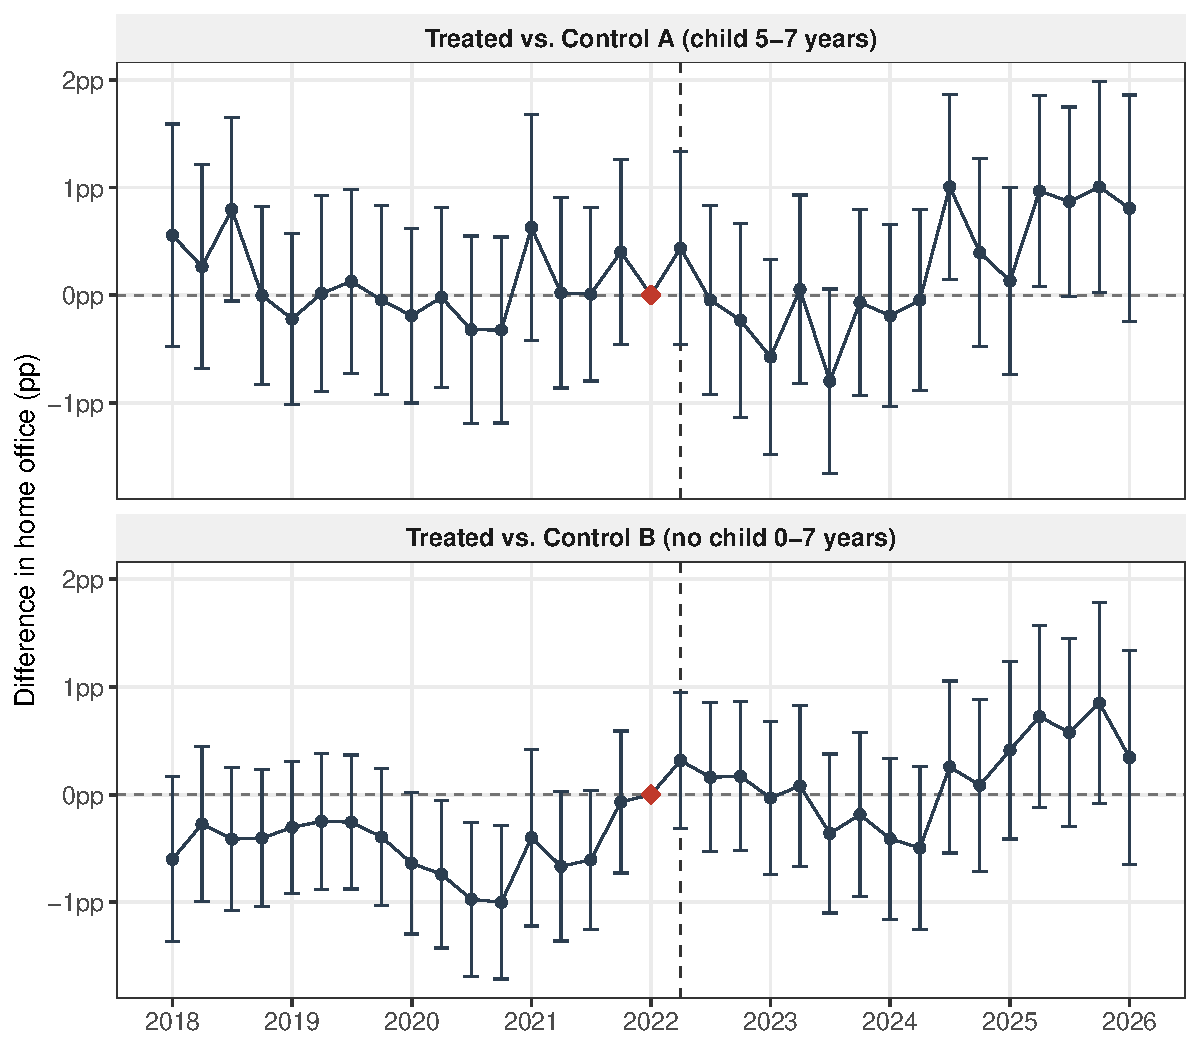
\includegraphics[width=0.85\textwidth]{fig06_event_study_home_office.pdf}
\caption{Event study: home office around the reform. Points are coefficients on the interaction of the treated indicator with each quarter, normalized to 2022Q1 (red marker); vertical bars are 95\% confidence intervals from household-clustered standard errors. The vertical dashed line marks the first post-reform quarter.}
\label{fig:event_home}
\end{figure}

\subsection{Reduced-form outcomes}

Table~\ref{tab:did_outcomes_A} reports the difference-in-differences estimates for the remaining outcomes using the primary comparison group. Real earnings and usual hours are statistically indistinguishable from zero. Employment and labor-force participation are estimated at about one percentage point with borderline significance, and maternity leave at about $-0.9$ points. These coefficients cannot be attributed to the reform: with a null first stage, the law's only channel---telework access---did not move, so any change in downstream outcomes must operate through some other mechanism or reflect trends unrelated to the policy. The maternity-leave estimate is a clear illustration. The corresponding event study (Appendix Figure~\ref{fig:event_maternity}) shows a strong pre-reform trend: the treated-versus-control gap in maternity leave was already declining well before 2022, so the parallel-trends assumption fails for that outcome and its coefficient is not interpreted causally. Home office, by contrast, is the one outcome with flat pre-trends, which is why the analysis centers on it. Finally, the placebo that compares the two control groups---mothers of children 5--7 versus women with no young children, neither of whom the law touches---is $+0.04$ points and insignificant, so the age threshold, rather than some generic difference between mothers and non-mothers, is what the design exploits.


\begin{table}[htbp]
   \caption{\label{tab:did_outcomes_A} Difference-in-Differences Estimates by Outcome, Control A}
   \centering
\footnotesize\setlength{\tabcolsep}{3pt}
   \begin{tabular}{lcccccc}
      \toprule
      Dependent Variables:     & Home office & Real income & Usual hours & Employed & In labor force & Maternity leave\\  
      Model:                   & (1)         & (2)         & (3)         & (4)      & (5)            & (6)\\  
      \midrule
      \emph{Variables}\\
      Treated (child $\leq$4)  & 0.003       & -22.3       & -0.244      & -0.009   & -0.007         & 0.013\\   
                               & (0.002)     & (25.9)      & (0.153)     & (0.004)  & (0.004)        & (0.002)\\   
      Treated $\times$ Post    & -0.0008     & 32.7        & 0.069       & 0.010    & 0.011          & -0.009\\   
                               & (0.003)     & (35.7)      & (0.202)     & (0.005)  & (0.005)        & (0.002)\\   
      \midrule
      \emph{Fixed-effects}\\
      Individual               & Yes         & Yes         & Yes         & Yes      & Yes            & Yes\\  
      Year-quarter             & Yes         & Yes         & Yes         & Yes      & Yes            & Yes\\  
      \midrule
      \emph{Fit statistics}\\
      Observations             & 989,898     & 481,352     & 504,745     & 989,898  & 989,898        & 989,898\\  
      R$^2$                    & 0.654       & 0.892       & 0.780       & 0.793    & 0.771          & 0.542\\  
\bottomrule
   \end{tabular}
   
   \par \raggedright 
   \footnotesize\textit{Notes:} Each column is a separate difference-in-differences regression under the preferred specification (treated main effect with individual and year-quarter fixed effects, weighted by the survey weights). Sample: women 18--49, household head or spouse, treated (child $\leq$4) vs.\ Control A (youngest child 5--7). Real income and usual hours are observed for workers only. Standard errors clustered at the household in parentheses. Significance levels: *** $p<0.01$, ** $p<0.05$, * $p<0.10$.
\end{table}




\subsection{Mechanisms}\label{sec:mechanisms}

If the reform had worked through the telework-priority channel, its effect on home office should have concentrated among women whose jobs can actually be done from home, and it might have induced eligible women to move toward such jobs. Neither is present in the data.

Table~\ref{tab:mech_moderation} splits the first stage by whether a woman was in a telework-eligible occupation at baseline, measured in her first observed quarter and held fixed so that it is not itself an outcome. The effect is no different from zero among the eligible---the only women for whom a priority in allocating telework positions could bind---and among the non-eligible. Table~\ref{tab:mech_allocation} takes the natural next step and uses telework eligibility of the current occupation as the outcome. A reform that pushed mothers to seek telework-friendly jobs in order to claim the priority would produce a positive coefficient; the estimate is essentially zero for both comparison groups. Appendix Table~\ref{tab:occ_transition} makes the same point descriptively: among women observed both before and after the reform, the pattern of occupation switches into and out of telework eligibility is nearly identical for treated and control mothers. There is, in short, no behavioral response of occupational choice to the priority.


\begin{table}[H]
   \caption{\label{tab:mech_moderation} First-Stage Home-Office Effect by Baseline Telework Eligibility}
   \centering
\small\setlength{\tabcolsep}{5pt}
   \begin{tabular}{lccc}
      \toprule
      Dependent Variable: & \multicolumn{3}{c}{Home office}\\
                                & All     & Telework-eligible & Not eligible \\   
      Model:                    & (1)     & (2)               & (3)\\  
      \midrule
      \emph{Variables}\\
      Treated (child $\leq$ 4)  & 0.003   & 0.003             & 0.003\\   
                                & (0.002) & (0.008)           & (0.002)\\   
\addlinespace[2pt]
      Treated $\times$ Post     & -0.0008 & -0.010            & 0.0005\\   
                                & (0.003) & (0.010)           & (0.003)\\   
\addlinespace[2pt]
      \midrule
      \emph{Fixed-effects}\\
      Individual                & Yes     & Yes               & Yes\\  
      Year-quarter              & Yes     & Yes               & Yes\\  
      \midrule
      \emph{Fit statistics}\\
      Observations              & 989,898 & 136,079           & 853,819\\  
      R$^2$                     & 0.654   & 0.713             & 0.633\\  
\bottomrule
   \end{tabular}
   
   \par \raggedright 
   \footnotesize\textit{Notes:} Each column estimates Eq.~\eqref{eq:did} (first stage, outcome home office) on the preferred sample (treated, child $\leq$ 4, vs.\ Control~A, youngest child 5--7), split by whether the woman was in a telework-eligible occupation at baseline---her occupation eligibility in her first observed quarter, held fixed, following \citet{costa2024}. All columns include individual and year-quarter fixed effects. All regressions are weighted by the survey weights. Standard errors are clustered at the household level in parentheses. Significance levels: *** $p<0.01$, ** $p<0.05$, * $p<0.10$.
\end{table}




\begin{table}[htbp]
   \caption{\label{tab:mech_allocation} Occupational Sorting: Telework-Eligible Occupation as Outcome}
   \centering
   \begin{tabular}{lcc}
      \tabularnewline \midrule \midrule
      Dependent Variable: & \multicolumn{2}{c}{Telework-eligible occ.}\\
                               & Control A (5--7) & Control B (no child 0--7) \\   
      Model:                   & (1)              & (2)\\  
      \midrule
      \emph{Variables}\\
      Treated (child $\leq$4)  & -0.001           & -0.010$^{***}$\\   
                               & (0.003)          & (0.003)\\   
      Treated $\times$ Post    & 0.0006           & -0.002\\   
                               & (0.003)          & (0.003)\\   
      \midrule
      \emph{Fixed-effects}\\
      Individual               & Yes              & Yes\\  
      Year-quarter             & Yes              & Yes\\  
      \midrule
      \emph{Fit statistics}\\
      Observations             & 989,898          & 2,192,875\\  
      R$^2$                    & 0.824            & 0.830\\  
      \midrule \midrule
      \multicolumn{3}{l}{\emph{Clustered (Household) standard-errors in parentheses}}\\
      \multicolumn{3}{l}{\emph{Signif. Codes: ***: 0.01, **: 0.05, *: 0.1}}\\
   \end{tabular}
   
   \par \raggedright 
   Outcome: indicator for being in a telework-eligible occupation. A positive Treated $\times$ Post means treated mothers move into eligible occupations after the reform. Same specification as the moderation table. $^{*}$/$^{**}$/$^{***}$: 10/5/1\%.
\end{table}




\subsection{Heterogeneity}\label{sec:heterogeneity}

Table~\ref{tab:heterogeneity} and Figure~\ref{fig:hetero} report the first-stage effect across subgroups, all defined at baseline. The splits by contract type are the most informative, because the statute binds only on registered private-sector employees: if the estimate reflected Article 75-F rather than a generic shock to mothers of young children, it should appear for that group and vanish for informal and public-sector workers. Instead it is indistinguishable from zero everywhere---for formal and informal workers, for registered private-sector employees and for public employees, and across education and age. Of the twelve subgroups only one, women aged forty to forty-nine, is individually significant; with twelve tests this is what one expects by chance, the group is small and selected, and there is no theory that would single it out. The heterogeneity analysis thus does not rescue a hidden effect; it shows the null is uniform, including where the law was supposed to bite hardest.

\begin{table}[H]\centering
\caption{Heterogeneity of the First-Stage Home-Office Effect}
\label{tab:heterogeneity}\small
\resizebox{\ifdim\width>\linewidth\linewidth\else\width\fi}{!}{%
\begin{tabular}{lcccc}
\toprule
 & Treated $\times$ Post (se) & $p$-value & Holm $p$ & Obs. \\
\midrule
\multicolumn{5}{l}{\textit{By formality}} \\
$\quad$ Formal & -0.03$^{}$ (0.50) & 0.950 & 1.00 & 261,866 \\
$\quad$ Informal & -0.13$^{}$ (0.38) & 0.727 & 1.00 & 728,032 \\
$\quad$ Private, signed card (CLT) & 0.27$^{}$ (0.65) & 0.681 & 1.00 & 152,995 \\
$\quad$ Non-CLT & -0.19$^{}$ (0.34) & 0.572 & 1.00 & 836,903 \\
\midrule
\multicolumn{5}{l}{\textit{By sector}} \\
$\quad$ Private employee & 0.18$^{}$ (0.58) & 0.752 & 1.00 & 197,959 \\
$\quad$ Public employee & -0.20$^{}$ (0.31) & 0.515 & 1.00 & 91,735 \\
\midrule
\multicolumn{5}{l}{\textit{By education}} \\
$\quad$ With higher education & 0.39$^{}$ (0.83) & 0.641 & 1.00 & 177,666 \\
$\quad$ Without higher education & -0.21$^{}$ (0.31) & 0.509 & 1.00 & 812,232 \\
\midrule
\multicolumn{5}{l}{\textit{By race}} \\
$\quad$ White & -0.20$^{}$ (0.50) & 0.693 & 1.00 & 341,737 \\
$\quad$ Non-white & 0.00$^{}$ (0.37) & 0.997 & 1.00 & 648,161 \\
\midrule
\multicolumn{5}{l}{\textit{By household structure}} \\
$\quad$ Single mother & -1.64$^{**}$ (0.73) & 0.024 & 0.36 & 159,369 \\
$\quad$ Partnered mother & 0.20$^{}$ (0.33) & 0.543 & 1.00 & 830,529 \\
\midrule
\multicolumn{5}{l}{\textit{Single mothers, by contract type}} \\
$\quad$ Single mother, CLT & 0.21$^{}$ (1.48) & 0.887 & --- & 24,588 \\
$\quad$ Single mother, non-CLT & -2.12$^{**}$ (0.83) & 0.010 & --- & 134,781 \\
\midrule
\multicolumn{5}{l}{\textit{By age band}} \\
$\quad$ Age 18--29 & -0.31$^{}$ (0.49) & 0.534 & 1.00 & 348,793 \\
$\quad$ Age 30--39 & -0.49$^{}$ (0.44) & 0.272 & 1.00 & 450,783 \\
$\quad$ Age 40--49 & 1.39$^{**}$ (0.69) & 0.042 & 0.59 & 190,322 \\
\bottomrule\end{tabular}}
\par\vspace{3pt}\footnotesize\raggedright \textit{Notes:} Each estimate is a separate first-stage difference-in-differences regression estimating Eq.~\eqref{eq:did} (outcome: home office, in percentage points) on the preferred sample (treated vs.\ Control~A), for the subgroup indicated; standard errors in parentheses next to the estimate. Subgroups are defined at baseline (first observed quarter); the ``Single mothers, by contract type'' rows decompose the single-mother cell and are not part of the Holm family (dash in the Holm-$p$ column). All regressions are weighted by the survey weights. Standard errors are clustered at the household level in parentheses. The Holm $p$ is the Holm step-down adjustment for testing the 15 subgroups, which controls the family-wise error rate under arbitrary dependence across the tests; a value of $1.00$ marks a subgroup far from significance. No subgroup is significant after adjustment: the smallest adjusted $p$-value is $0.36$ (the ``Single mother'' subgroup). Significance levels: *** $p<0.01$, ** $p<0.05$, * $p<0.10$.
\end{table}


\begin{figure}[H]
\centering
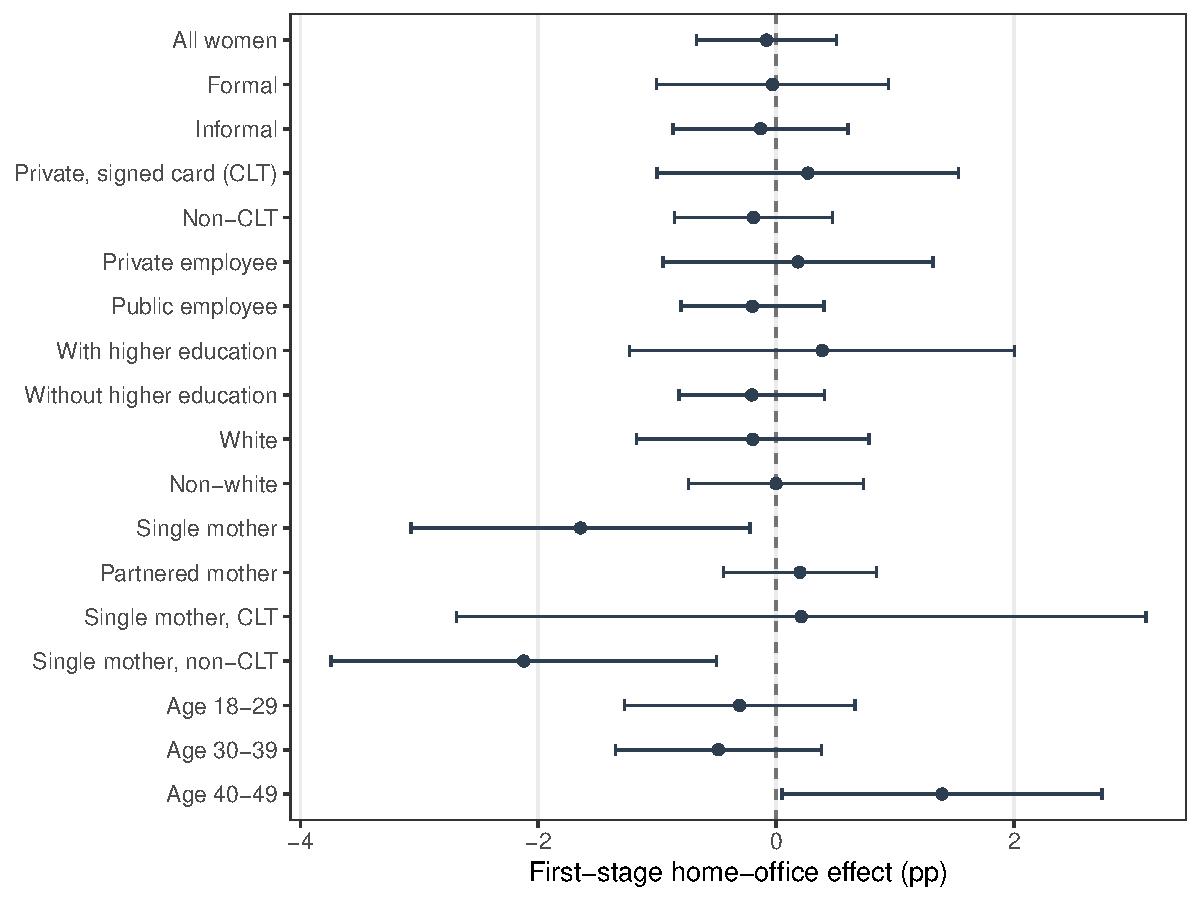
\includegraphics[width=0.85\textwidth]{fig07_heterogeneity_coefplot.pdf}
\caption{First-stage home-office effect by subgroup. Points are difference-in-differences estimates; horizontal bars are 95\% confidence intervals from household-clustered standard errors. Subgroups are defined at baseline.}
\label{fig:hetero}
\end{figure}

\subsection{Robustness and a triple difference}\label{sec:robustness}

Table~\ref{tab:robustness} collects robustness checks on the first stage. The null is unchanged when the post-period starts one quarter earlier, when the treatment definition excludes grandchildren or stepchildren, when the pandemic years are dropped so that a clean 2018--2019 pre-period is compared with the post-reform quarters, when the sample is restricted to prime childbearing ages, when state-by-quarter fixed effects absorb region-specific shocks, when standard errors are clustered two ways, and when the sample is limited to telework-eligible occupations. A control-window robustness (Appendix Figure~\ref{fig:window}) widens the comparison group from a youngest child aged 5--6 up to 5--12 and finds the estimate stable throughout. Earnings tell the same story: measured in logs among workers with positive pay, the effect is a precise zero, and it is unchanged when earnings are winsorized at the 99th percentile.

\begin{table}[htbp]\centering
\caption{Robustness of the First-Stage Home-Office Effect}
\label{tab:robustness}\small
\begin{tabular}{lcc}
\toprule
 & Treated $\times$ Post & Obs. \\
\midrule
\multicolumn{3}{l}{\textit{Home office (pp)}} \\
Baseline & -0.08$^{}$ & 1,020,823 \\
 & (0.30) & \\
Alternative cutoff (2022Q1 post) & 0.20$^{}$ & 1,020,823 \\
 & (0.30) & \\
Treated excl.\ grandchildren & -0.07$^{}$ & 956,777 \\
 & (0.31) & \\
Treated excl.\ stepchildren & -0.13$^{}$ & 1,005,187 \\
 & (0.30) & \\
Excluding 2020--2021 (COVID) & -0.09$^{}$ & 823,117 \\
 & (0.37) & \\
Ages 20--35 & -0.36$^{}$ & 617,885 \\
 & (0.38) & \\
Ages 20--40 & -0.41$^{}$ & 830,421 \\
 & (0.33) & \\
State $\times$ quarter fixed effects & -0.08$^{}$ & 1,020,823 \\
 & (0.30) & \\
Two-way cluster (household, PSU) & -0.08$^{}$ & 1,020,823 \\
 & (0.29) & \\
Matched panel only & -0.08$^{}$ & 989,898 \\
 & (0.30) & \\
Telework-eligible only & -0.95$^{}$ & 139,496 \\
 & (1.01) & \\
\midrule
\multicolumn{3}{l}{\textit{Real income (R\$), outlier sensitivity}} \\
Income: raw & 32.7$^{}$ & 495,994 \\
 & (35.7) & \\
Income: winsor. 1\% & 5.3$^{}$ & 495,994 \\
 & (26.8) & \\
\bottomrule\end{tabular}
\par\vspace{3pt}\footnotesize\raggedright \textit{Notes:} Each estimate is a separate difference-in-differences regression on the preferred sample (treated vs.\ Control A, child 5--7), including the treated main effect, individual and year-quarter fixed effects, and survey weights; standard errors clustered at the household in parentheses (except the two-way row, clustered at the household and primary sampling unit). $^{*}$/$^{**}$/$^{***}$ denote significance at 10/5/1\%. The placebo on men is reported in Table \ref{tab:triple_diff}.
\end{table}


Because Article 75-F is not gender-restricted, men with young children are also eligible, which allows a triple difference that nets out any generic shock to parents of young children after 2022 and isolates the woman-specific response. Table~\ref{tab:triple_diff} reports the first stage for men and women separately and the triple-difference coefficient. Men show no effect either, the women's estimate is the null already reported, and the triple-difference term is small and insignificant: the absence of an effect is not gendered. Appendix Table~\ref{tab:triple_diff_outcomes} extends the triple difference to the other outcomes; the significant coefficients there track the pre-existing gender-differential trends discussed above rather than the reform.


\begin{table}[htbp]
   \caption{\label{tab:triple_diff} Triple Difference: Home Office, Men vs.\ Women}
   \centering
   \begin{tabular}{lccc}
      \tabularnewline \midrule \midrule
      Dependent Variable: & \multicolumn{3}{c}{Home office}\\
                                              & Men           & Women     & DDD \\   
      Model:                                  & (1)           & (2)       & (3)\\  
      \midrule
      \emph{Variables}\\
      Treated (child $\leq$4)                 & -0.004$^{**}$ & 0.003     & -0.004$^{**}$\\   
                                              & (0.002)       & (0.002)   & (0.002)\\   
      Treated $\times$ Post                   & 0.002         & -0.0008   & 0.002\\   
                                              & (0.002)       & (0.003)   & (0.002)\\   
      Treated $\times$ Female                 &               &           & 0.007$^{***}$\\   
                                              &               &           & (0.003)\\   
      Treated $\times$ Post $\times$ Female   &               &           & -0.003\\   
                                              &               &           & (0.004)\\   
      \midrule
      \emph{Fixed-effects}\\
      Individual                              & Yes           & Yes       & Yes\\  
      Year-quarter                            & Yes           & Yes       & \\  
      Female-Year-quarter                     &               &           & Yes\\  
      \midrule
      \emph{Fit statistics}\\
      Observations                            & 798,373       & 1,020,823 & 1,819,196\\  
      R$^2$                                   & 0.673         & 0.662     & 0.666\\  
      \midrule \midrule
      \multicolumn{4}{l}{\emph{Clustered (Household) standard-errors in parentheses}}\\
      \multicolumn{4}{l}{\emph{Signif. Codes: ***: 0.01, **: 0.05, *: 0.1}}\\
   \end{tabular}
   
   \par \raggedright 
   Columns 1--2 are separate DiDs for men and women (treated $=$ child $\leq$4 vs.\ Control A). Column 3 is the pooled triple difference; the coefficient Treated $\times$ Post $\times$ Female is the extra effect for women relative to men, with female$\times$year-quarter fixed effects absorbing any sex-specific time shock. Individual FE throughout; weighted; SE clustered at the household. $^{*}$/$^{**}$/$^{***}$: 10/5/1\%.
\end{table}




% =============================================================================
\section{Discussion}\label{sec:discussion}
% =============================================================================

The central finding is a precisely estimated null: a legal priority to telework for mothers of young children did not raise their telework take-up, and produced no detectable change in occupational sorting or labor-market outcomes. The most plausible reading is institutional. Article 75-F grants a priority in allocation, not a right to telework: the employer must place eligible employees ahead of others when distributing positions that are already teleworkable, but is under no obligation to create such positions or to grant remote work to anyone in particular, and the provision carries no enforcement mechanism or penalty. A priority is therefore only as valuable as the stock of teleworkable positions an employer has to allocate and its willingness to reallocate them---and for most eligible women that stock is close to empty.

The population the mandate can reach is narrow. The statute binds on registered private-sector employees under the CLT, yet a large share of Brazilian women work informally or are outside formal employment, where the provision does not apply; among the formally employed, only a minority hold occupations that can plausibly be performed from home. Home office is correspondingly rare---about 5\% of employed women in the sample---so even a mandate that bound perfectly among the teleworkable would move the population average little. Consistent with this, the effect is no larger among women who were already in telework-eligible occupations, the subgroup for whom a priority in allocating telework positions is not vacuous, and there is no sign that eligible mothers moved toward such occupations to claim the benefit.

Two further explanations, familiar from the mandated-benefits literature, likely reinforce the null. First, workers are often unaware of workplace entitlements and may neither request nor act on them; a priority that is never invoked imposes no cost on employers and prompts no reallocation. Second, where telework is feasible, employers who could offer it to a mother of a young child were largely already free to do so, so a non-binding legal preference adds little at the margin. The event study is consistent with a slow and, at most, modest adjustment: any movement appears only two to three years after enactment, once the measure had been converted into permanent law, rather than as a sharp break at the reform date.

Two limitations qualify the interpretation. The estimates are intent-to-treat effects of eligibility, not of telework itself, and are silent about the women who did obtain remote work; the true effect on that group is larger, though it is bounded above by the near-zero first stage. And the sample runs through early 2026: the small, late upward drift in the event study could reflect a genuine slow-moving response that additional post-reform data would sharpen or dispel. On the evidence available, however, the mandate did not move the outcome it targeted.

% =============================================================================
\section{Conclusion}\label{sec:conclusion}
% =============================================================================

Brazil's 2022 reform gave mothers of young children a legal priority in the allocation of remote-work positions. Using the rotating panel of the national household survey and a difference-in-differences design built around the statutory age-4 threshold, I find that the reform did not raise the share of eligible women working from home. The estimate is a precise zero; it is robust to the fixed-effects specification, to the definition of treatment and controls, to the pandemic window, to clustering, and to the choice of comparison group; it is uniform across subgroups, including the registered private-sector employees the law binds; and it is accompanied by no occupational sorting toward telework-eligible jobs and no gendered pattern in a triple difference. The result is a caution for a policy instrument that is cheap, increasingly popular, and easy to legislate: expanding access to workplace flexibility, and through it narrowing gender gaps, appears to require more than instructing employers to prefer one group over another.

\clearpage
\bibliography{refs}

\clearpage
\appendix
% =============================================================================
% appendix.tex — inputted by paper.tex after \appendix
% =============================================================================

\section{The PNADC and the advanced panel identification}\label{app:pnadc}

\paragraph{The survey.} The Continuous National Household Sample Survey (\emph{Pesquisa Nacional por Amostra de Domicílios Cont\'inua}, PNADC) is the household labor-force survey conducted by the Brazilian Institute of Geography and Statistics (IBGE). It is a stratified, multi-stage probability sample of the resident population, released quarterly, and is the source of Brazil's official labor-market statistics. The survey follows a rotating panel scheme: each selected household is interviewed in 5 consecutive quarters and then leaves the sample. As a result, a given household, and the individuals in it, can be observed up to 5 times over roughly 15 months, which provides the short longitudinal dimension exploited in this paper. Because the sample is not self-weighting, all estimates use the survey's calibrated sampling weights, and the design information is retained for variance estimation. The outcome used as the first stage, the location at which a worker performs her main job, has been collected since the first quarter of 2018, which sets the start of the estimation window.

\paragraph{Linking individuals across quarters.} The public microdata do not contain a permanent personal identifier, so respondents must be linked across quarters from the information that is available: the household's position in the sample rotation, the ordering of individuals within the household, and demographic characteristics such as sex and date of birth. When interviews are complete and consistent, this linkage is straightforward. In practice a non-trivial share of interviews contain small inconsistencies, such as a missing or misrecorded birth date or a change in the reported household roster, that break naive matches. I use an advanced identification procedure that reconstructs the panel in the presence of such inconsistencies by treating the linkage as a graph-matching problem, in which candidate records are connected when they are compatible on the stable identifiers and demographic characteristics and the most consistent set of links is selected. Individuals that the procedure cannot confidently match are assigned a singleton identifier and therefore contribute nothing to the within-person variation that identifies the fixed-effects estimates. The estimation sample is accordingly restricted to confidently matched individuals; the roughly 3.7\% of women who cannot be linked are excluded. Because the excluded observations are singletons, this restriction changes the number of observations but leaves the fixed-effects estimates numerically unchanged.

\paragraph{Panel quality.} Table~\ref{tab:panel_retention} documents that the reconstructed panel captures genuine repeated observations rather than spurious matches. It reports, for the estimation sample, the share of households and of matched individuals observed for at least a given number of quarters, together with the quarter-to-quarter continuation probability. The figures are computed on the analysis sample, prime-age women who head a household or are the head's spouse, and so reflect both survey attrition and the sample definition: a woman who ages out of the 18--49 window, or a household that no longer contains a qualifying woman, leaves the sample even though the survey continues to interview her. This is why retention is lower than an unrestricted population figure would be; it is a feature of the sample definition, not a failure of the matching. The key point for the identification is that a substantial share of women are observed repeatedly, so that individual fixed effects are meaningful.

\input{../analysis/output/tables/tabA0_panel_retention.tex}

\clearpage
\section{Additional tables and figures}\label{app:additional}

Table~\ref{tab:robustness} collects the robustness checks on the first stage discussed in Section~\ref{sec:robustness}, and Figure~\ref{fig:hetero} summarizes the subgroup estimates of Table~\ref{tab:heterogeneity} as a coefficient plot. Table~\ref{tab:did_outcomes_B} repeats the difference-in-differences estimates using the broad comparison group (women with no child aged 0--7), which delivers more precision at the cost of a less tightly matched counterfactual; the conclusions are unchanged. Figure~\ref{fig:event_maternity} shows the event study for maternity leave, which exhibits the pronounced pre-reform trend discussed in the text and motivates treating that outcome as non-causal. Table~\ref{tab:occ_transition} reports the occupation-transition matrix underlying the mechanism discussion. Table~\ref{tab:triple_diff_outcomes} extends the triple difference to all outcomes. Figure~\ref{fig:window} reports the control-window robustness.

\begin{table}[htbp]\centering
\caption{Robustness of the First-Stage Home-Office Effect}
\label{tab:robustness}\small
\begin{tabular}{lcc}
\toprule
 & Treated $\times$ Post & Obs. \\
\midrule
\multicolumn{3}{l}{\textit{Home office (pp)}} \\
Baseline & -0.08$^{}$ & 1,020,823 \\
 & (0.30) & \\
Alternative cutoff (2022Q1 post) & 0.20$^{}$ & 1,020,823 \\
 & (0.30) & \\
Treated excl.\ grandchildren & -0.07$^{}$ & 956,777 \\
 & (0.31) & \\
Treated excl.\ stepchildren & -0.13$^{}$ & 1,005,187 \\
 & (0.30) & \\
Excluding 2020--2021 (COVID) & -0.09$^{}$ & 823,117 \\
 & (0.37) & \\
Ages 20--35 & -0.36$^{}$ & 617,885 \\
 & (0.38) & \\
Ages 20--40 & -0.41$^{}$ & 830,421 \\
 & (0.33) & \\
State $\times$ quarter fixed effects & -0.08$^{}$ & 1,020,823 \\
 & (0.30) & \\
Two-way cluster (household, PSU) & -0.08$^{}$ & 1,020,823 \\
 & (0.29) & \\
Matched panel only & -0.08$^{}$ & 989,898 \\
 & (0.30) & \\
Telework-eligible only & -0.95$^{}$ & 139,496 \\
 & (1.01) & \\
\midrule
\multicolumn{3}{l}{\textit{Real income (R\$), outlier sensitivity}} \\
Income: raw & 32.7$^{}$ & 495,994 \\
 & (35.7) & \\
Income: winsor. 1\% & 5.3$^{}$ & 495,994 \\
 & (26.8) & \\
\bottomrule\end{tabular}
\par\vspace{3pt}\footnotesize\raggedright \textit{Notes:} Each estimate is a separate difference-in-differences regression on the preferred sample (treated vs.\ Control A, child 5--7), including the treated main effect, individual and year-quarter fixed effects, and survey weights; standard errors clustered at the household in parentheses (except the two-way row, clustered at the household and primary sampling unit). $^{*}$/$^{**}$/$^{***}$ denote significance at 10/5/1\%. The placebo on men is reported in Table \ref{tab:triple_diff}.
\end{table}


\begin{figure}[H]
\centering
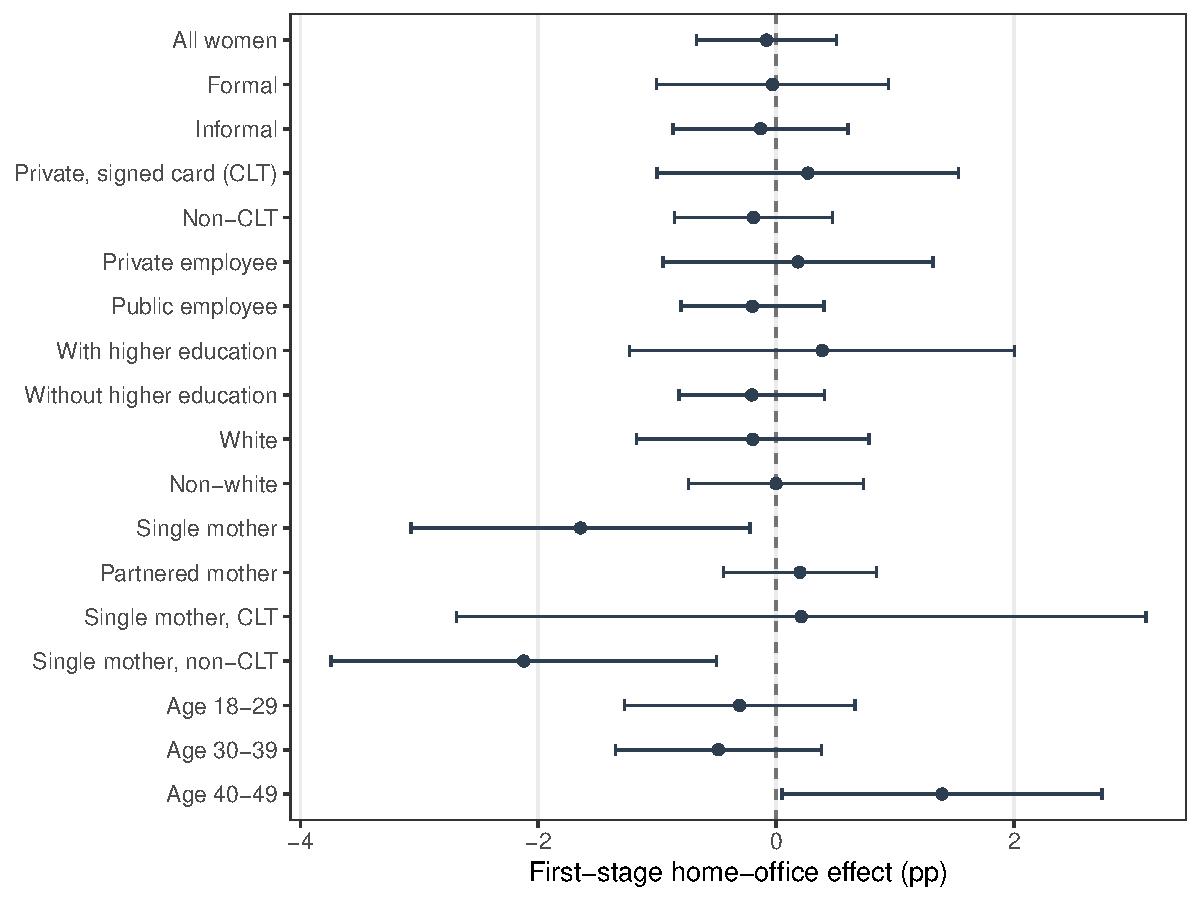
\includegraphics[width=0.85\textwidth]{fig07_heterogeneity_coefplot.pdf}
\caption{First-stage home-office effect by subgroup. Points are difference-in-differences estimates and horizontal bars are 95\% confidence intervals from household-clustered standard errors. Subgroups are defined at baseline.}
\label{fig:hetero}
\end{figure}


\begin{table}[H]
   \caption{\label{tab:did_outcomes_B} Difference-in-Differences Estimates by Outcome, Control B}
   \centering
\footnotesize\setlength{\tabcolsep}{3pt}
   \begin{tabular}{lcccccc}
      \toprule
      Dependent Variables:     & Home office & Real income & Usual hours    & Employed       & In labor force & Maternity leave\\  
      Model:                   & (1)         & (2)         & (3)            & (4)            & (5)            & (6)\\  
      \midrule
      \emph{Variables}\\
      Treated (child $\leq$4)  & -0.003      & -20.3       & -0.645$^{***}$ & -0.065$^{***}$ & -0.071$^{***}$ & 0.114$^{***}$\\   
                               & (0.002)     & (36.4)      & (0.177)        & (0.004)        & (0.004)        & (0.004)\\   
\addlinespace[2pt]
      Treated $\times$ Post    & 0.004       & 14.3        & -0.093         & 0.008$^{*}$    & 0.008$^{**}$   & -0.011$^{***}$\\   
                               & (0.003)     & (39.5)      & (0.177)        & (0.004)        & (0.004)        & (0.002)\\   
\addlinespace[2pt]
      \midrule
      \emph{Fixed-effects}\\
      Individual               & Yes         & Yes         & Yes            & Yes            & Yes            & Yes\\  
      Year-quarter             & Yes         & Yes         & Yes            & Yes            & Yes            & Yes\\  
      \midrule
      \emph{Fit statistics}\\
      Observations             & 2,192,875   & 1,251,406   & 1,302,376      & 2,192,875      & 2,192,875      & 2,192,875\\  
      R$^2$                    & 0.664       & 0.889       & 0.765          & 0.797          & 0.778          & 0.475\\  
\bottomrule
   \end{tabular}
   
   \par \raggedright 
   \footnotesize\textit{Notes:} As in the Control~A outcome table, using the broad comparison group (women with no child aged 0--7). Each column is a separate difference-in-differences regression under the preferred specification (treated main effect with individual and year-quarter fixed effects, weighted by the survey weights). Home office, employed, in labor force, and maternity leave are 0/1 indicators, so a coefficient of $0.01$ corresponds to one percentage point; real income is in reais per month and usual hours in hours per week, both observed for workers only. Standard errors clustered at the household in parentheses. Significance levels: *** $p<0.01$, ** $p<0.05$, * $p<0.10$.
\end{table}




\begin{figure}[H]
\centering
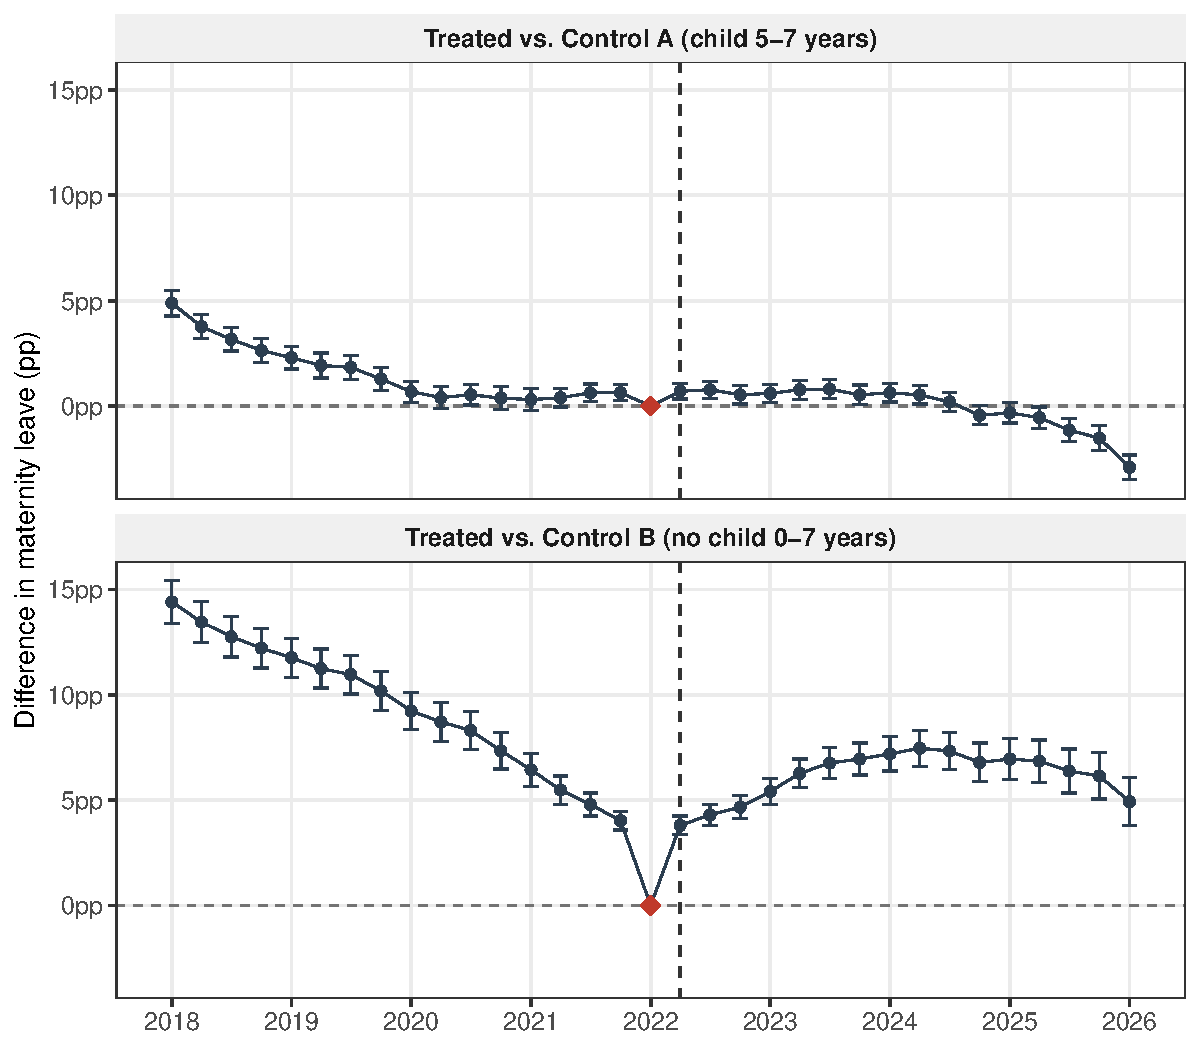
\includegraphics[width=0.82\textwidth]{fig09_event_study_maternity.pdf}
\caption{Event study: maternity leave around the reform. Constructed exactly as Figure~\ref{fig:event_home}. The pronounced pre-reform trend in the treated-versus-control gap indicates that the parallel-trends assumption fails for this outcome, which is therefore not interpreted causally.}
\label{fig:event_maternity}
\end{figure}

\begin{table}[H]\centering
\caption{Occupation Transitions Around the Reform}
\label{tab:occ_transition}\small
\begin{tabular}{lcc}
\toprule
\multicolumn{3}{l}{\textit{Treated (child $\leq$4)}} \\
 & Post: not eligible & Post: eligible \\
$\quad$ Pre: not eligible & 84.3\% & 3.5\% \\
$\quad$ Pre: eligible & 2.6\% & 9.5\% \\
\midrule
\multicolumn{3}{l}{\textit{Control A (child 5--7)}} \\
 & Post: not eligible & Post: eligible \\
$\quad$ Pre: not eligible & 82.4\% & 3.7\% \\
$\quad$ Pre: eligible & 2.7\% & 11.1\% \\
\bottomrule\end{tabular}
\par\vspace{3pt}\footnotesize\raggedright \textit{Notes:} Each cell is the share of women in a given pre-to-post telework-eligibility transition, among matched women observed both before and after the second quarter of 2022 (15,048 treated and 6,587 control women). Off-diagonal cells are occupation switches. The treated and control distributions are similar, consistent with the null in Table~\ref{tab:mech_allocation}.
\end{table}


\begin{table}[htbp]
   \caption{\label{tab:triple_diff_outcomes} Triple Difference Across Outcomes}
   \centering
   \begin{tabular}{lcccccc}
      \tabularnewline \midrule \midrule
      Dependent Variables:                    & Home office   & Real income   & Usual hours & Employed  & In labor force & Maternity leave\\  
      Model:                                  & (1)           & (2)           & (3)         & (4)       & (5)            & (6)\\  
      \midrule
      \emph{Variables}\\
      Treated (child $\leq$4)                 & -0.004$^{**}$ & -40.2         & 0.040       & -0.0006   & 0.005$^{**}$   & 0.0002\\   
                                              & (0.002)       & (42.0)        & (0.118)     & (0.003)   & (0.002)        & (0.0002)\\   
      Treated $\times$ Female                 & 0.007$^{***}$ & 18.2          & -0.287      & -0.009    & -0.012$^{**}$  & 0.013$^{***}$\\   
                                              & (0.003)       & (44.5)        & (0.181)     & (0.006)   & (0.005)        & (0.002)\\   
      Treated $\times$ Post                   & 0.002         & 161.8$^{***}$ & 0.129       & 0.005     & -0.0006        & -0.0002\\   
                                              & (0.002)       & (58.0)        & (0.148)     & (0.004)   & (0.003)        & (0.0002)\\   
      Treated $\times$ Post $\times$ Female   & -0.003        & -129.6$^{**}$ & -0.054      & 0.005     & 0.011$^{**}$   & -0.008$^{***}$\\   
                                              & (0.004)       & (60.7)        & (0.237)     & (0.006)   & (0.006)        & (0.002)\\   
      \midrule
      \emph{Fixed-effects}\\
      Individual                              & Yes           & Yes           & Yes         & Yes       & Yes            & Yes\\  
      Female-Year-quarter                     & Yes           & Yes           & Yes         & Yes       & Yes            & Yes\\  
      \midrule
      \emph{Fit statistics}\\
      Observations                            & 1,819,196     & 1,202,578     & 1,228,429   & 1,819,196 & 1,819,196      & 1,819,196\\  
      R$^2$                                   & 0.666         & 0.887         & 0.759       & 0.802     & 0.795          & 0.546\\  
      \midrule \midrule
      \multicolumn{7}{l}{\emph{Clustered (Household) standard-errors in parentheses}}\\
      \multicolumn{7}{l}{\emph{Signif. Codes: ***: 0.01, **: 0.05, *: 0.1}}\\
   \end{tabular}
   
   \par \raggedright 
   Each column is a triple-difference regression with the same specification as the first-stage triple difference. Reported: the men effect (Treated $\times$ Post) and the female differential (Treated $\times$ Post $\times$ Female). $^{*}$/$^{**}$/$^{***}$: 10/5/1\%.
\end{table}




\begin{figure}[H]
\centering
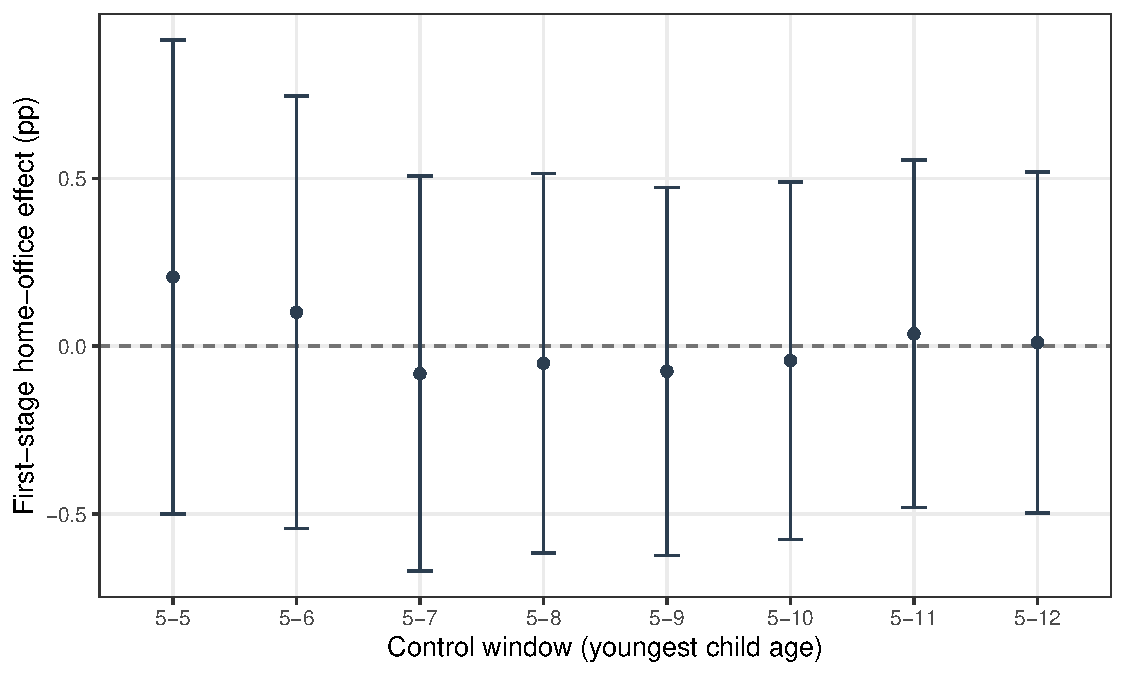
\includegraphics[width=0.8\textwidth]{fig08_control_window_sweep.pdf}
\caption{Control-window robustness. Each point is the first-stage difference-in-differences estimate as the comparison group is widened from a youngest child aged 5--6 up to 5--12; bars are 95\% confidence intervals. The estimate is stable across windows.}
\label{fig:window}
\end{figure}


\end{document}
